\documentclass[10pt]{article}
\usepackage[T1]{fontenc}
\usepackage{lmodern}
\usepackage{float}
\usepackage[utf8]{inputenc}
\usepackage[letterpaper,margin=2.3cm]{geometry}
\usepackage{amsmath,amssymb}
\usepackage{array,booktabs,longtable,graphicx,caption}
\usepackage{xurl}
\usepackage[hidelinks]{hyperref}
\captionsetup{font=small,labelfont=bf}
\renewcommand{\thetable}{S\arabic{table}}
\renewcommand{\thefigure}{S\arabic{figure}}
\renewcommand{\thesection}{S\arabic{section}}
\setlength{\LTcapwidth}{\textwidth}
\binoppenalty=10000 \relpenalty=10000 % no partir fórmulas en + o = (S1)
\pagestyle{plain}
\begin{document}

\begin{center}
{\Large\bfseries Supplementary Material\par}\vspace{4pt}
{\itshape A Benchmark of Five Machine-Learning Architectures for Daily Trading-Signal Classification on US Tech Equities\par}\vspace{3pt}
{\small MICAI 2026 --- Lecture Notes in Artificial Intelligence --- Chapter 171490174\par}
\end{center}
\vspace{4pt}

\noindent This document contains the material that the paper refers to as ``supplementary
material''. Each section corresponds to one reference in the paper. The results in Sections S2--S4
come from the benchmark reported in Section~7 of the paper (120 runs, test year 2025); for the sequence models
(LSTM, CNN~1D and CNN-LSTM) the reported run is the better of the two look-backs (20 or 60 days)
by test F1-macro, as in the paper. They reproduce Tables~4, 5 and~6 of the paper.

\section{Full list of the 61 input features (paper \S3.3)}
All features are computed per ticker from daily OHLCV data adjusted for splits and dividends
($O,H,L,C,V$) and, for the last family, from SPY and the CBOE VIX, using only information
available at the close of day~$t$. Column names are those used in the code.

\begin{longtable}{@{}r l >{\raggedright\arraybackslash}p{0.66\textwidth}@{}}
\caption{Input features, grouped by family (count in parentheses).}\label{tab:s1}\\
\toprule \# & Column & Definition \\ \midrule \endfirsthead
\toprule \# & Column & Definition \\ \midrule \endhead
\bottomrule \endlastfoot
\multicolumn{3}{@{}l}{\emph{Log returns} (5)} \\*[1pt]
1 & \texttt{ret\_1d} & $\ln(C_t/C_{t-1})$ \\
2 & \texttt{ret\_2d} & $\ln(C_t/C_{t-2})$ \\
3 & \texttt{ret\_3d} & $\ln(C_t/C_{t-3})$ \\
4 & \texttt{ret\_5d} & $\ln(C_t/C_{t-5})$ \\
5 & \texttt{ret\_10d} & $\ln(C_t/C_{t-10})$ \\
\midrule
\multicolumn{3}{@{}l}{\emph{Momentum} (4)} \\*[1pt]
6 & \texttt{mom\_5d} & $C_t/C_{t-4}-1$ \\
7 & \texttt{mom\_10d} & $C_t/C_{t-9}-1$ \\
8 & \texttt{mom\_20d} & $C_t/C_{t-19}-1$ \\
9 & \texttt{mom\_60d} & $C_t/C_{t-59}-1$ \\
\midrule
\multicolumn{3}{@{}l}{\emph{Moving averages} (9)} \\*[1pt]
10 & \texttt{dist\_ma10} & $C_t/\mathrm{MA}_{10}-1$, with $\mathrm{MA}_k$ the $k$-day simple moving average of $C$ \\
11 & \texttt{dist\_ma20} & $C_t/\mathrm{MA}_{20}-1$ \\
12 & \texttt{dist\_ma30} & $C_t/\mathrm{MA}_{30}-1$ \\
13 & \texttt{dist\_ma50} & $C_t/\mathrm{MA}_{50}-1$ \\
14 & \texttt{dist\_ma200} & $C_t/\mathrm{MA}_{200}-1$ \\
15 & \texttt{cruce\_ma10\_ma50} & $\mathrm{MA}_{10}/\mathrm{MA}_{50}-1$ (crossover) \\
16 & \texttt{cruce\_ma20\_ma50} & $\mathrm{MA}_{20}/\mathrm{MA}_{50}-1$ (crossover) \\
17 & \texttt{cruce\_ma50\_ma200} & $\mathrm{MA}_{50}/\mathrm{MA}_{200}-1$ (crossover) \\
18 & \texttt{pendiente\_ma20} & $(\mathrm{MA}_{20,t}-\mathrm{MA}_{20,t-5})/\mathrm{MA}_{20,t-5}$ (slope) \\
\midrule
\multicolumn{3}{@{}l}{\emph{Volatility} (8)} \\*[1pt]
19 & \texttt{atr\_14} & ATR(14): 14-day mean of $\mathrm{TR}_t=\max(H-L,\,|H-C_{t-1}|,\,|L-C_{t-1}|)$ \\
20 & \texttt{atr\_norm} & $\mathrm{ATR}(14)/C_t$ \\
21 & \texttt{vol\_5d} & $\mathrm{std}_5(\text{ret\_1d})\sqrt{252}$ \\
22 & \texttt{vol\_10d} & $\mathrm{std}_{10}(\text{ret\_1d})\sqrt{252}$ \\
23 & \texttt{vol\_20d} & $\mathrm{std}_{20}(\text{ret\_1d})\sqrt{252}$ \\
24 & \texttt{vol\_60d} & $\mathrm{std}_{60}(\text{ret\_1d})\sqrt{252}$ \\
25 & \texttt{vol\_ratio\_5\_20} & vol\_5d / vol\_20d \\
26 & \texttt{vol\_ratio\_20\_60} & vol\_20d / vol\_60d \\
\midrule
\multicolumn{3}{@{}l}{\emph{Oscillators} (9)} \\*[1pt]
27 & \texttt{rsi\_14} & Wilder RSI(14): $100-100/(1+\overline{\text{gain}}/\overline{\text{loss}})$, exponential smoothing $\alpha=1/14$ \\
28 & \texttt{rsi\_7} & Wilder RSI(7), $\alpha=1/7$ \\
29 & \texttt{macd} & $(\mathrm{EMA}_{12}(C)-\mathrm{EMA}_{26}(C))/C_t$ \\
30 & \texttt{macd\_sig} & $\mathrm{EMA}_9(\text{MACD line})/C_t$ \\
31 & \texttt{macd\_hist} & $(\text{MACD line}-\text{signal line})/C_t$ \\
32 & \texttt{stoch\_k} & $\%K=100\,(C-\min_{14}L)/(\max_{14}H-\min_{14}L)$ \\
33 & \texttt{stoch\_d} & $\%D$: 3-day mean of $\%K$ \\
34 & \texttt{stoch\_diff} & $\%K-\%D$ \\
35 & \texttt{williams\_r} & $-100\,(\max_{14}H-C)/(\max_{14}H-\min_{14}L)$ \\
\midrule
\multicolumn{3}{@{}l}{\emph{Volume and flow} (8)} \\*[1pt]
36 & \texttt{vol\_log} & $\ln(V+1)$ \\
37 & \texttt{vol\_ratio} & $V_t/\mathrm{MA}_{20}(V)$ \\
38 & \texttt{obv\_ratio} & $\mathrm{OBV}_t/|\mathrm{MA}_{20}(\mathrm{OBV})|-1$, $\mathrm{OBV}_t=\sum\mathrm{sign}(\Delta C)\,V$ from the first downloaded day \\
39 & \texttt{obv\_pendiente} & $\big((\mathrm{OBV}_t-\mathrm{OBV}_{t-5})/\mathrm{OBV}_{t-5}\big)/C_t$ (OBV slope) \\
40 & \texttt{vwap\_dist} & $(C-\mathrm{VWAP}_{20})/\mathrm{VWAP}_{20}$, $\mathrm{VWAP}_{20}=\sum_{20}\mathrm{TP}\,V/\sum_{20}V$, $\mathrm{TP}=(H+L+C)/3$ \\
41 & \texttt{cmf\_20} & Chaikin money flow $\sum_{20}\mathrm{CLV}\,V/\sum_{20}V$, $\mathrm{CLV}=((C-L)-(H-C))/(H-L)$ \\
42 & \texttt{mfi\_14} & Money flow index over 14 days on $\mathrm{TP}\,V$ \\
43 & \texttt{vol\_trend} & $\mathrm{MA}_{20}(V)/\mathrm{MA}_{60}(V)-1$ \\
\midrule
\multicolumn{3}{@{}l}{\emph{Candle patterns} (7)} \\*[1pt]
44 & \texttt{rango\_rel} & $(H-L)/C$ (relative range) \\
45 & \texttt{cambio\_intra} & $(C-O)/O$ (intraday change) \\
46 & \texttt{cuerpo\_rel} & $|C-O|/(H-L)$ (body / range) \\
47 & \texttt{sombra\_sup} & $(H-\max(O,C))/\mathrm{ATR}(14)$ (upper shadow) \\
48 & \texttt{sombra\_inf} & $(\min(O,C)-L)/\mathrm{ATR}(14)$ (lower shadow) \\
49 & \texttt{gap\_apertura} & $(O_t-C_{t-1})/C_{t-1}$ (opening gap) \\
50 & \texttt{hl\_ratio} & $(C-L)/(H-L)$ (position of the close in the range) \\
\midrule
\multicolumn{3}{@{}l}{\emph{Seasonality} (5)} \\*[1pt]
51 & \texttt{dia\_sin} & $\sin(2\pi d/5)$, $d$ = weekday (Monday $=0$) \\
52 & \texttt{dia\_cos} & $\cos(2\pi d/5)$ \\
53 & \texttt{mes\_sin} & $\sin(2\pi m/12)$, $m$ = month (1--12) \\
54 & \texttt{mes\_cos} & $\cos(2\pi m/12)$ \\
55 & \texttt{semana\_mes} & $(w-2.5)/2.5$, $w=\lfloor(\text{day of month}-1)/7\rfloor+1$ \\
\midrule
\multicolumn{3}{@{}l}{\emph{Market context} (6)} \\*[1pt]
56 & \texttt{SP500\_ret} & $\ln(\mathrm{SPY}_t/\mathrm{SPY}_{t-1})$ \\
57 & \texttt{SP500\_vol20} & $\mathrm{std}_{20}(\text{SP500\_ret})\sqrt{252}$ \\
58 & \texttt{SP500\_mom20} & $\mathrm{SPY}_t/\mathrm{SPY}_{t-19}-1$ \\
59 & \texttt{VIX} & close of the CBOE VIX index (\texttt{\textasciicircum VIX}) \\
60 & \texttt{VIX\_change} & $\mathrm{VIX}_t/\mathrm{VIX}_{t-1}-1$ \\
61 & \texttt{VIX\_norm} & $(\mathrm{VIX}-\mathrm{MA}_{252}(\mathrm{VIX}))/\mathrm{std}_{252}(\mathrm{VIX})$ \\
\end{longtable}

\section{Per-class F1 for every run (paper \S5.1)}
F1-macro and per-class F1 on the 2025 test set for the 120 runs (5 models $\times$
3 experiments $\times$ (1 global + 7 per-ticker)). ``Global'' models are trained on the seven
tickers together and scored on all of them; per-ticker models are trained and scored on one
ticker. Look-back is the number of past days given to the sequence models.

{\small\begin{longtable}{@{}l l c c c c c c@{}}
\caption{Test F1-macro and per-class F1 of the 120 runs (test year 2025).}\label{tab:s2}\\
\toprule Model & Training & Exp & Look-back & F1-macro & F1 SELL & F1 HOLD & F1 BUY \\ \midrule \endfirsthead
\toprule Model & Training & Exp & Look-back & F1-macro & F1 SELL & F1 HOLD & F1 BUY \\ \midrule \endhead
\bottomrule \endlastfoot
LR & Global & A & -- & 0.411 & 0.357 & 0.521 & 0.354 \\
LR & Global & B & -- & 0.385 & 0.364 & 0.512 & 0.278 \\
LR & Global & C & -- & 0.401 & 0.355 & 0.533 & 0.314 \\
LR & AAPL & A & -- & 0.394 & 0.352 & 0.514 & 0.315 \\
LR & AAPL & B & -- & 0.384 & 0.333 & 0.528 & 0.290 \\
LR & AAPL & C & -- & 0.369 & 0.306 & 0.483 & 0.317 \\
LR & NVDA & A & -- & 0.418 & 0.410 & 0.549 & 0.296 \\
LR & NVDA & B & -- & 0.421 & 0.405 & 0.598 & 0.261 \\
LR & NVDA & C & -- & 0.299 & 0.418 & 0.479 & 0.000 \\
LR & TSLA & A & -- & 0.408 & 0.428 & 0.492 & 0.303 \\
LR & TSLA & B & -- & 0.360 & 0.406 & 0.475 & 0.198 \\
LR & TSLA & C & -- & 0.359 & 0.396 & 0.422 & 0.258 \\
LR & AMZN & A & -- & 0.423 & 0.410 & 0.500 & 0.358 \\
LR & AMZN & B & -- & 0.430 & 0.469 & 0.523 & 0.297 \\
LR & AMZN & C & -- & 0.386 & 0.473 & 0.447 & 0.237 \\
LR & MSFT & A & -- & 0.408 & 0.315 & 0.568 & 0.340 \\
LR & MSFT & B & -- & 0.376 & 0.288 & 0.554 & 0.286 \\
LR & MSFT & C & -- & 0.382 & 0.339 & 0.562 & 0.246 \\
LR & GOOGL & A & -- & 0.420 & 0.279 & 0.602 & 0.378 \\
LR & GOOGL & B & -- & 0.384 & 0.387 & 0.461 & 0.302 \\
LR & GOOGL & C & -- & 0.358 & 0.408 & 0.396 & 0.271 \\
LR & META & A & -- & 0.410 & 0.353 & 0.462 & 0.414 \\
LR & META & B & -- & 0.387 & 0.254 & 0.548 & 0.358 \\
LR & META & C & -- & 0.357 & 0.194 & 0.495 & 0.383 \\
\midrule
XGBoost & Global & A & -- & 0.396 & 0.357 & 0.486 & 0.346 \\
XGBoost & Global & B & -- & 0.386 & 0.367 & 0.453 & 0.338 \\
XGBoost & Global & C & -- & 0.373 & 0.353 & 0.426 & 0.341 \\
XGBoost & AAPL & A & -- & 0.384 & 0.336 & 0.529 & 0.286 \\
XGBoost & AAPL & B & -- & 0.336 & 0.325 & 0.426 & 0.257 \\
XGBoost & AAPL & C & -- & 0.339 & 0.306 & 0.434 & 0.275 \\
XGBoost & NVDA & A & -- & 0.380 & 0.362 & 0.474 & 0.304 \\
XGBoost & NVDA & B & -- & 0.338 & 0.324 & 0.400 & 0.291 \\
XGBoost & NVDA & C & -- & 0.372 & 0.392 & 0.482 & 0.241 \\
XGBoost & TSLA & A & -- & 0.406 & 0.340 & 0.497 & 0.382 \\
XGBoost & TSLA & B & -- & 0.441 & 0.385 & 0.505 & 0.435 \\
XGBoost & TSLA & C & -- & 0.395 & 0.317 & 0.461 & 0.408 \\
XGBoost & AMZN & A & -- & 0.352 & 0.309 & 0.374 & 0.374 \\
XGBoost & AMZN & B & -- & 0.390 & 0.363 & 0.419 & 0.389 \\
XGBoost & AMZN & C & -- & 0.377 & 0.367 & 0.404 & 0.361 \\
XGBoost & MSFT & A & -- & 0.425 & 0.381 & 0.492 & 0.403 \\
XGBoost & MSFT & B & -- & 0.399 & 0.387 & 0.436 & 0.372 \\
XGBoost & MSFT & C & -- & 0.331 & 0.327 & 0.419 & 0.248 \\
XGBoost & GOOGL & A & -- & 0.344 & 0.258 & 0.419 & 0.354 \\
XGBoost & GOOGL & B & -- & 0.336 & 0.286 & 0.394 & 0.329 \\
XGBoost & GOOGL & C & -- & 0.328 & 0.328 & 0.385 & 0.271 \\
XGBoost & META & A & -- & 0.342 & 0.323 & 0.366 & 0.336 \\
XGBoost & META & B & -- & 0.347 & 0.271 & 0.400 & 0.370 \\
XGBoost & META & C & -- & 0.321 & 0.290 & 0.314 & 0.359 \\
\midrule
LSTM & Global & A & 60 & 0.389 & 0.371 & 0.522 & 0.274 \\
LSTM & Global & B & 60 & 0.370 & 0.286 & 0.522 & 0.301 \\
LSTM & Global & C & 20 & 0.370 & 0.281 & 0.473 & 0.356 \\
LSTM & AAPL & A & 60 & 0.358 & 0.121 & 0.528 & 0.424 \\
LSTM & AAPL & B & 20 & 0.383 & 0.286 & 0.557 & 0.306 \\
LSTM & AAPL & C & 20 & 0.322 & 0.078 & 0.459 & 0.429 \\
LSTM & NVDA & A & 20 & 0.154 & 0.375 & 0.000 & 0.087 \\
LSTM & NVDA & B & 20 & 0.328 & 0.250 & 0.635 & 0.099 \\
LSTM & NVDA & C & 20 & 0.277 & 0.370 & 0.462 & 0.000 \\
LSTM & TSLA & A & 20 & 0.202 & 0.057 & 0.111 & 0.439 \\
LSTM & TSLA & B & 60 & 0.291 & 0.267 & 0.254 & 0.353 \\
LSTM & TSLA & C & 20 & 0.299 & 0.057 & 0.465 & 0.374 \\
LSTM & AMZN & A & 20 & 0.351 & 0.209 & 0.438 & 0.405 \\
LSTM & AMZN & B & 20 & 0.335 & 0.216 & 0.386 & 0.404 \\
LSTM & AMZN & C & 20 & 0.363 & 0.216 & 0.533 & 0.341 \\
LSTM & MSFT & A & 20 & 0.392 & 0.447 & 0.455 & 0.273 \\
LSTM & MSFT & B & 20 & 0.353 & 0.436 & 0.483 & 0.139 \\
LSTM & MSFT & C & 60 & 0.332 & 0.346 & 0.547 & 0.102 \\
LSTM & GOOGL & A & 20 & 0.380 & 0.265 & 0.503 & 0.372 \\
LSTM & GOOGL & B & 60 & 0.415 & 0.234 & 0.571 & 0.439 \\
LSTM & GOOGL & C & 20 & 0.377 & 0.115 & 0.600 & 0.416 \\
LSTM & META & A & 20 & 0.359 & 0.323 & 0.432 & 0.324 \\
LSTM & META & B & 60 & 0.364 & 0.336 & 0.420 & 0.337 \\
LSTM & META & C & 60 & 0.310 & 0.383 & 0.252 & 0.295 \\
\midrule
CNN-LSTM & Global & A & 60 & 0.376 & 0.277 & 0.492 & 0.360 \\
CNN-LSTM & Global & B & 20 & 0.384 & 0.273 & 0.546 & 0.331 \\
CNN-LSTM & Global & C & 60 & 0.371 & 0.266 & 0.525 & 0.323 \\
CNN-LSTM & AAPL & A & 20 & 0.353 & 0.284 & 0.487 & 0.288 \\
CNN-LSTM & AAPL & B & 60 & 0.325 & 0.215 & 0.494 & 0.266 \\
CNN-LSTM & AAPL & C & 20 & 0.307 & 0.052 & 0.529 & 0.339 \\
CNN-LSTM & NVDA & A & 20 & 0.302 & 0.365 & 0.542 & 0.000 \\
CNN-LSTM & NVDA & B & 20 & 0.311 & 0.300 & 0.633 & 0.000 \\
CNN-LSTM & NVDA & C & 20 & 0.339 & 0.410 & 0.546 & 0.060 \\
CNN-LSTM & TSLA & A & 20 & 0.413 & 0.277 & 0.535 & 0.427 \\
CNN-LSTM & TSLA & B & 20 & 0.352 & 0.426 & 0.395 & 0.235 \\
CNN-LSTM & TSLA & C & 20 & 0.383 & 0.357 & 0.469 & 0.321 \\
CNN-LSTM & AMZN & A & 60 & 0.384 & 0.200 & 0.569 & 0.384 \\
CNN-LSTM & AMZN & B & 20 & 0.418 & 0.375 & 0.523 & 0.357 \\
CNN-LSTM & AMZN & C & 20 & 0.378 & 0.286 & 0.472 & 0.376 \\
CNN-LSTM & MSFT & A & 20 & 0.370 & 0.272 & 0.526 & 0.311 \\
CNN-LSTM & MSFT & B & 20 & 0.329 & 0.368 & 0.562 & 0.058 \\
CNN-LSTM & MSFT & C & 20 & 0.380 & 0.305 & 0.510 & 0.325 \\
CNN-LSTM & GOOGL & A & 60 & 0.391 & 0.275 & 0.571 & 0.326 \\
CNN-LSTM & GOOGL & B & 20 & 0.315 & 0.000 & 0.613 & 0.333 \\
CNN-LSTM & GOOGL & C & 20 & 0.343 & 0.385 & 0.566 & 0.079 \\
CNN-LSTM & META & A & 20 & 0.361 & 0.348 & 0.546 & 0.188 \\
CNN-LSTM & META & B & 20 & 0.346 & 0.356 & 0.476 & 0.207 \\
CNN-LSTM & META & C & 20 & 0.360 & 0.398 & 0.524 & 0.160 \\
\midrule
CNN 1D & Global & A & 60 & 0.361 & 0.221 & 0.532 & 0.329 \\
CNN 1D & Global & B & 20 & 0.343 & 0.113 & 0.515 & 0.402 \\
CNN 1D & Global & C & 20 & 0.373 & 0.288 & 0.507 & 0.323 \\
CNN 1D & AAPL & A & 20 & 0.295 & 0.305 & 0.232 & 0.347 \\
CNN 1D & AAPL & B & 20 & 0.363 & 0.226 & 0.545 & 0.318 \\
CNN 1D & AAPL & C & 60 & 0.159 & 0.000 & 0.113 & 0.363 \\
CNN 1D & NVDA & A & 60 & 0.409 & 0.378 & 0.503 & 0.345 \\
CNN 1D & NVDA & B & 20 & 0.316 & 0.000 & 0.576 & 0.373 \\
CNN 1D & NVDA & C & 20 & 0.286 & 0.404 & 0.454 & 0.000 \\
CNN 1D & TSLA & A & 20 & 0.408 & 0.403 & 0.436 & 0.385 \\
CNN 1D & TSLA & B & 20 & 0.406 & 0.270 & 0.585 & 0.362 \\
CNN 1D & TSLA & C & 60 & 0.314 & 0.236 & 0.364 & 0.343 \\
CNN 1D & AMZN & A & 20 & 0.371 & 0.209 & 0.507 & 0.397 \\
CNN 1D & AMZN & B & 20 & 0.325 & 0.093 & 0.534 & 0.348 \\
CNN 1D & AMZN & C & 20 & 0.282 & 0.000 & 0.571 & 0.275 \\
CNN 1D & MSFT & A & 20 & 0.387 & 0.260 & 0.516 & 0.386 \\
CNN 1D & MSFT & B & 60 & 0.279 & 0.000 & 0.564 & 0.274 \\
CNN 1D & MSFT & C & 20 & 0.286 & 0.049 & 0.523 & 0.286 \\
CNN 1D & GOOGL & A & 20 & 0.379 & 0.127 & 0.535 & 0.474 \\
CNN 1D & GOOGL & B & 60 & 0.328 & 0.387 & 0.598 & 0.000 \\
CNN 1D & GOOGL & C & 60 & 0.336 & 0.091 & 0.515 & 0.403 \\
CNN 1D & META & A & 60 & 0.396 & 0.420 & 0.443 & 0.325 \\
CNN 1D & META & B & 20 & 0.304 & 0.000 & 0.556 & 0.357 \\
CNN 1D & META & C & 20 & 0.297 & 0.355 & 0.424 & 0.111 \\
\end{longtable}}

\section{Economic metrics for Exps A and C (paper \S7.1)}
Same metrics as Table~5 of the paper (which reports Exp~B) for the global models of the other two
experiments: long on BUY, short on SELL, flat on HOLD, one-day holding period, no transaction
costs; Sharpe is annualized. Best value per column in bold.

\begin{table}[H]\centering
\caption{Economic metrics, Exp A (10 training years) GLOBAL, test = 2025.}\label{tab:s3}
\begin{tabular}{@{}lccccc@{}}\toprule
Model & F1 & Win rate & Profit factor & Max drawdown & Sharpe \\ \midrule
LR & {\boldmath\textbf{0.411}} & {\boldmath\textbf{0.528}} & {\boldmath\textbf{1.296}} & $-0.551$ & {\boldmath\textbf{$+1.067$}} \\
XGBoost & 0.396 & 0.505 & 1.143 & $-0.464$ & $+0.575$ \\
LSTM & 0.389 & 0.510 & 1.284 & $-0.392$ & $+0.965$ \\
CNN-LSTM & 0.376 & 0.502 & 1.187 & $-0.460$ & $+0.686$ \\
CNN 1D & 0.361 & 0.467 & 1.007 & {\boldmath\textbf{$-0.365$}} & $+0.025$ \\
\bottomrule\end{tabular}\end{table}
\begin{table}[H]\centering
\caption{Economic metrics, Exp C (4 training years) GLOBAL, test = 2025.}\label{tab:s4}
\begin{tabular}{@{}lccccc@{}}\toprule
Model & F1 & Win rate & Profit factor & Max drawdown & Sharpe \\ \midrule
LR & {\boldmath\textbf{0.401}} & {\boldmath\textbf{0.513}} & {\boldmath\textbf{1.297}} & $-0.445$ & {\boldmath\textbf{$+1.023$}} \\
XGBoost & 0.373 & 0.500 & 1.090 & {\boldmath\textbf{$-0.428$}} & $+0.377$ \\
LSTM & 0.370 & 0.496 & 1.039 & $-0.631$ & $+0.163$ \\
CNN-LSTM & 0.371 & 0.508 & 1.182 & $-0.463$ & $+0.624$ \\
CNN 1D & 0.373 & 0.494 & 0.924 & $-0.666$ & $-0.317$ \\
\bottomrule\end{tabular}\end{table}

\section{Sharpe ratio by model and ticker (paper \S7.3)}
\begin{figure}[H]\centering
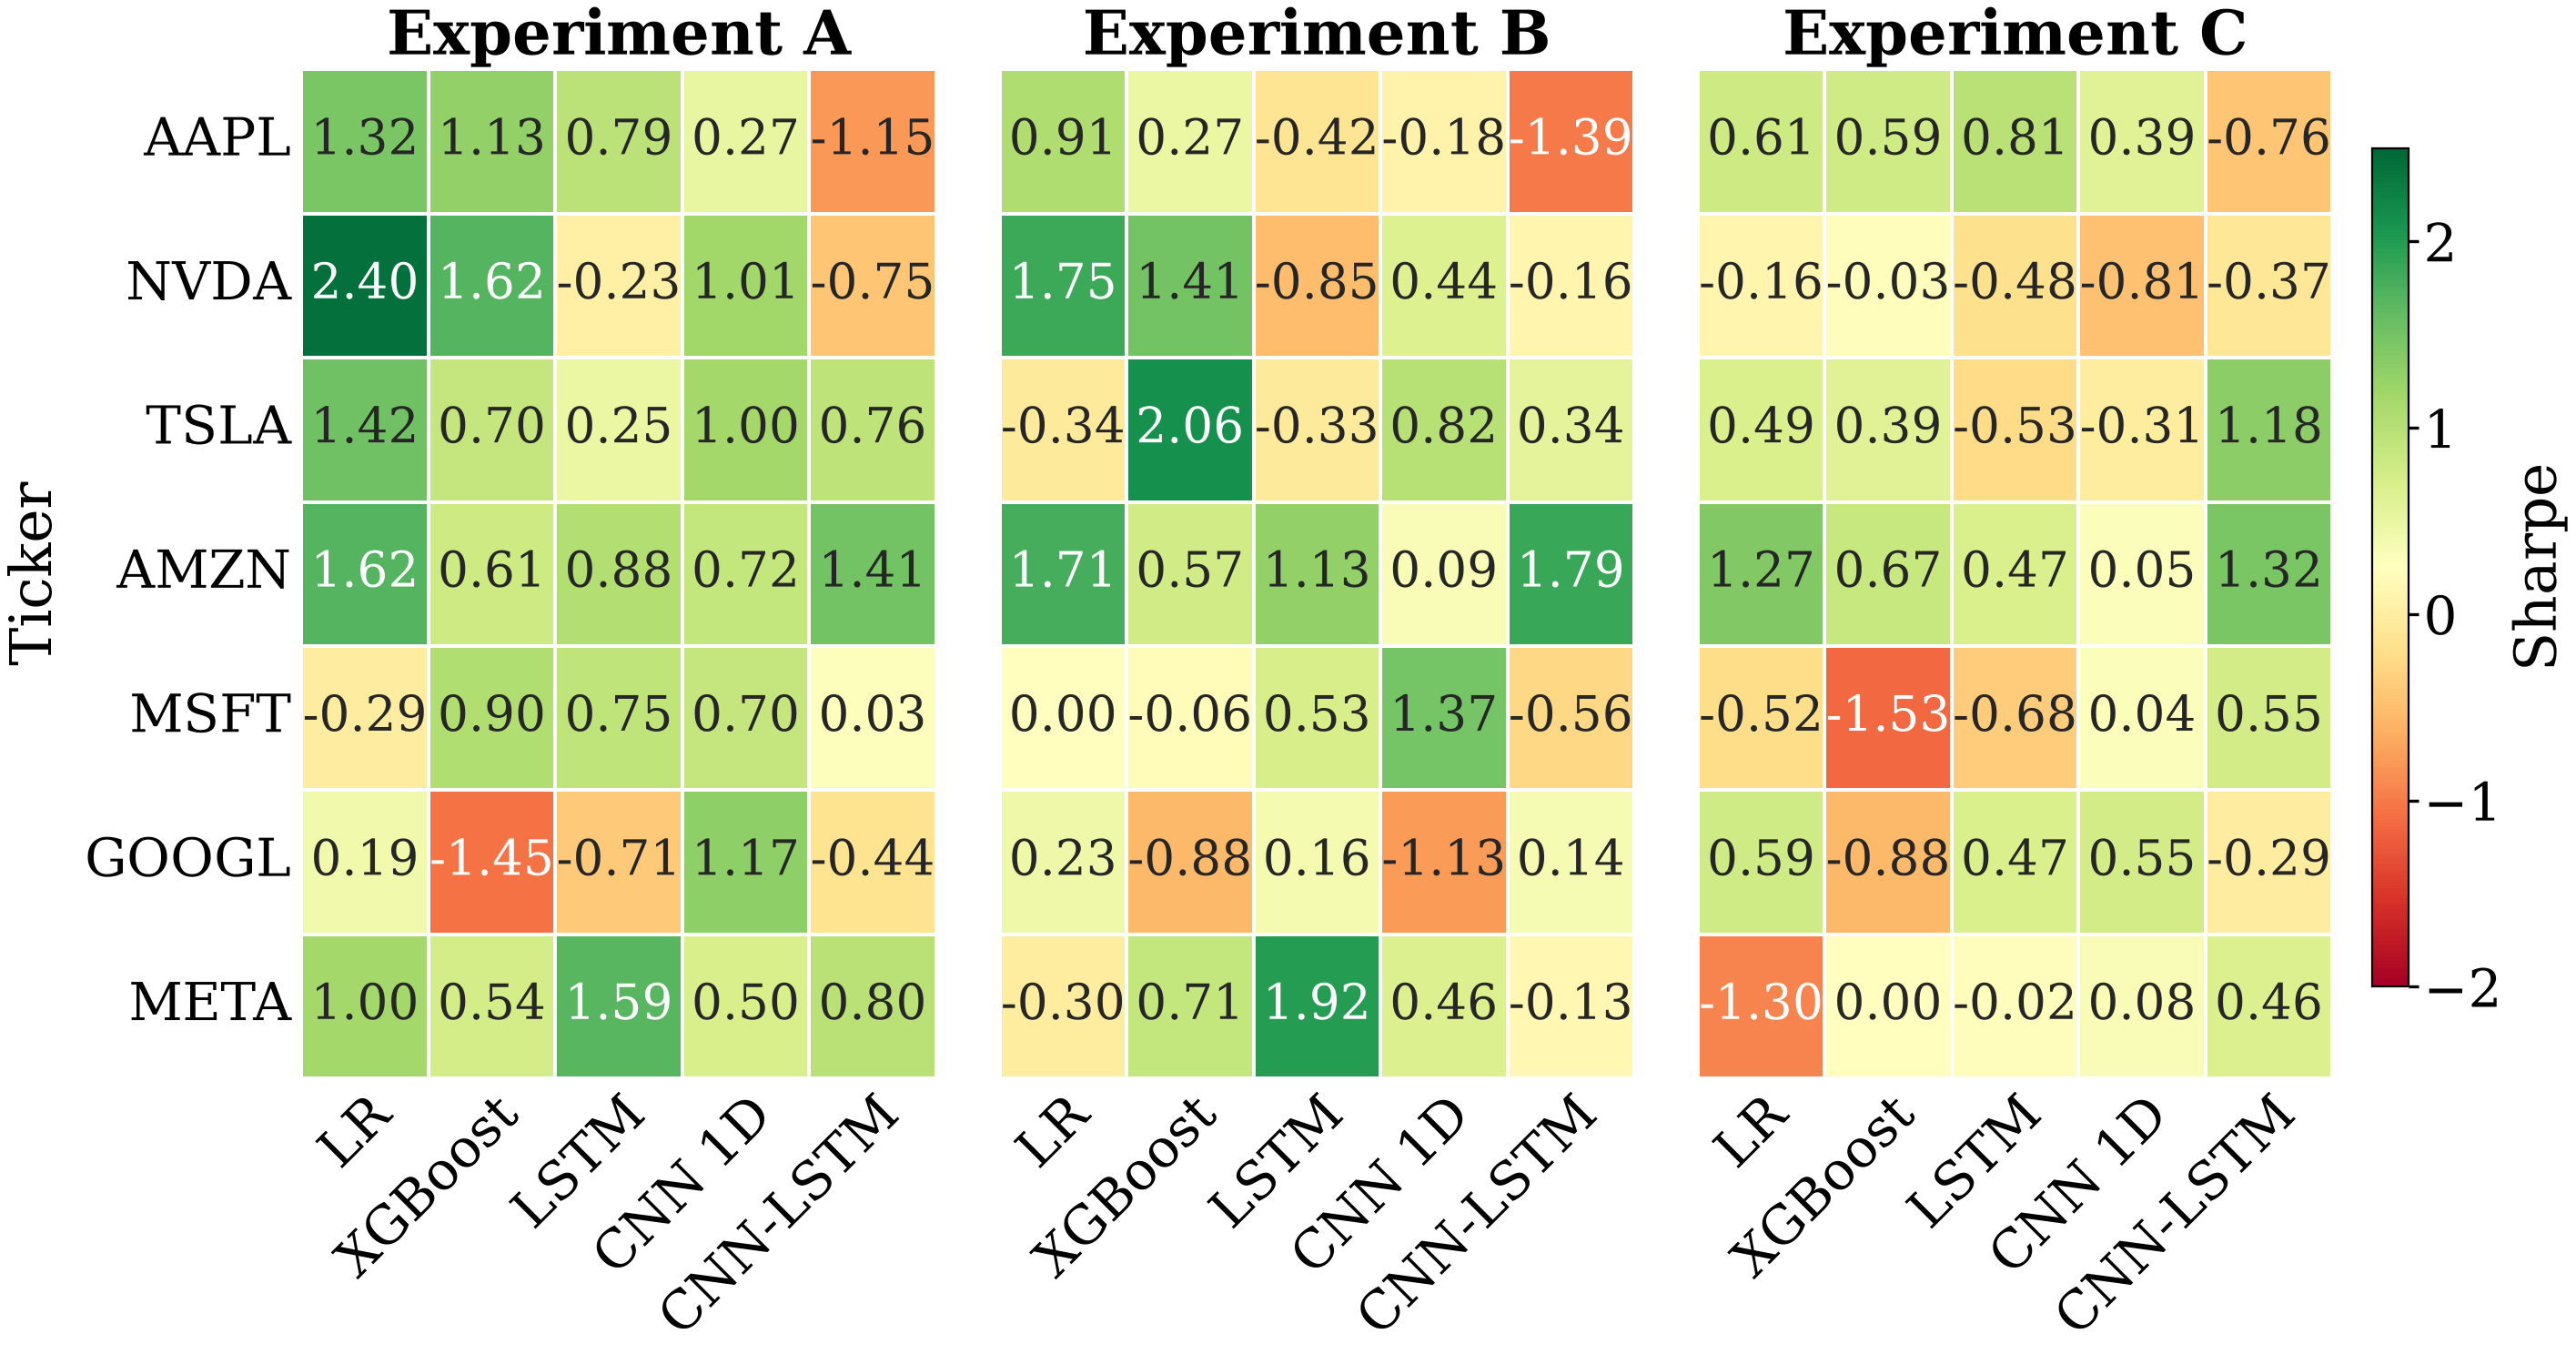
\includegraphics[width=0.92\textwidth]{fig_sharpe_heatmap.png}
\caption{Annualized Sharpe ratio of the per-ticker models, per model and ticker, for the three
experiments (test = 2025). These are the 105 values whose variance decomposition is given in
Section~7.3 of the paper.}\label{fig:s1}
\end{figure}

\section{Code, data manifest, random seeds and library versions (paper \S11)}
\paragraph{Code.} The complete pipeline is publicly available at \url{https://github.com/barudust/TT}; a snapshot
of the repository for this paper is tagged \texttt{micai2026} (\url{https://github.com/barudust/TT/tree/micai2026}).
Table~\ref{tab:code} lists where each part of the paper is implemented.

\begin{table}[H]\centering\small
\caption{Where each part of the paper is implemented (paths relative to the repository root).}\label{tab:code}
\begin{tabular}{@{}p{0.34\textwidth}p{0.6\textwidth}@{}}\toprule
Part of the paper & Files \\ \midrule
\S3 Data download, features and label & \path{scripts_v1/01_build_raw_dataset.py} \\
\S3.4 Temporal splits & \path{scripts_opt/common_v4.py} \\
\S6 Statistical feature pre-selection & \path{scripts_opt/analisis_feature_selection.py} \\
\S7 Benchmark of 120 runs & \path{scripts_opt/train_all_v4.py} \newline \path{scripts_opt/consolidar_v4.py} \newline \path{RESULTADOS_OPTIMIZADOS/v4/resultados_v4.csv} (results) \\
\S8 Robustness study & \path{scripts_opt/run_v5.py} \newline \path{scripts_opt/common_v5.py} \newline \path{scripts_opt/reporte_v5.py} \newline \path{RESULTADOS_OPTIMIZADOS/v5/} (results) \\
Figures & \path{scripts_opt/plots_paper.py} \\
Reproduction checks & \path{RESULTADOS_OPTIMIZADOS/v5/g0_replicacion.csv} (results) \newline \path{scripts_opt/replicar_lr_v4.py} \newline \path{RESULTADOS_OPTIMIZADOS/v4/replica_lr_v4.csv} (results) \\
This document & \path{paper_review/supplementary/build_supplementary.py} \\
\bottomrule\end{tabular}\end{table}

\paragraph{Data manifest.} Source: Yahoo Finance through the \texttt{yfinance} library, daily
bars adjusted for splits and dividends (\texttt{auto\_adjust=True}), downloaded for 2013-01-01 to
2025-12-31; the first year serves as warm-up for the indicators. Market context: SPY and \texttt{\textasciicircum VIX}
over the same window. Label: one-day forward log-return; BUY if it reaches the 70th percentile and
SELL if it falls to the 30th percentile of the previous 252 trading days of the same ticker
(thresholds shifted by one day, so no future information enters them), HOLD otherwise. Rows per
ticker: training 2,516 (Exp~A, 2014--2023), 1,509 (Exp~B, 2018--2023) and 1,006 (Exp~C,
2020--2023); validation 252 (2024); test 248 (2025). Global models use the seven tickers together
(1,736 test rows); in Section~7 the sequence models were scored on the test days with a complete
look-back window (1,596 rows at look-back 20 and 1,316 at 60), which the protocol of Section~8
aligns to the same 1,736 rows. Table~\ref{tab:s5} lists the stored datasets.

\begin{table}[H]\centering
\caption{Stored datasets \texttt{tesis\_ml\_stocks/01\_raw\_datasets/\textless TICKER\textgreater\_raw.parquet} (one row per trading day: the 61 features, the raw OHLCV, and the label with its forward return and percentile thresholds) and their SHA-256 checksums.}\label{tab:s5}
\begin{tabular}{@{}lcccl@{}}\toprule
Ticker & First day & Last day & Rows & SHA-256 \\ \midrule
AAPL & 2013-12-31 & 2025-12-29 & 3,017 & {\scriptsize\texttt{fe020d29efa861c96dad12a5d7e2070bcc876e5db3146ec6b8083ec69df3d2eb}} \\
NVDA & 2013-12-31 & 2025-12-29 & 3,017 & {\scriptsize\texttt{6e5afa41aacb7556402f391bd07460f1aaba5695f5cada58042278766ac86b0c}} \\
TSLA & 2013-12-31 & 2025-12-29 & 3,017 & {\scriptsize\texttt{83535218b012e791db6fa6b60a8f4459b0ee6a14541c53203b74edd03fc7d6e0}} \\
AMZN & 2013-12-31 & 2025-12-29 & 3,017 & {\scriptsize\texttt{70518ea782bd65bb7b5fb10147c026a4c8bd7ff83255f51baa0565764d386300}} \\
MSFT & 2013-12-31 & 2025-12-29 & 3,017 & {\scriptsize\texttt{22bd02e399884a6e06399def52f2cef2e2d1cc5ab9e6402d288a0ce2dbaa5db4}} \\
GOOGL & 2013-12-31 & 2025-12-29 & 3,017 & {\scriptsize\texttt{fc19f91c45c0c524ebaaa93be82f28a31befd62a8fbf8dc89a2cea256eebba5c}} \\
META & 2013-12-31 & 2025-12-29 & 3,017 & {\scriptsize\texttt{9fc4d44cc1913040225335329b332102f19bb3ddd97a7646fdf0b68318e69780}} \\
\bottomrule\end{tabular}\end{table}

\paragraph{Random seeds.} Benchmark (\S7): LR is trained with seeds $\{42, 1, 7, 2024, 100\}$ and
the final class is the majority vote of the five models; XGBoost, LSTM, CNN~1D and CNN-LSTM are
trained with seeds $\{42, 1, 7\}$ and their class probabilities are averaged; the Optuna search of
XGBoost uses a TPE sampler with seed~42. Robustness study (\S8): Optuna TPE sampler with seed~42
(25 random start-up trials) and a median pruner for the deep models; every frozen configuration is
evaluated on the test year with seeds $\{42, 1, 7, 2024, 100\}$.

\paragraph{Library versions and hardware.} PyTorch~2.12 (CUDA~12.8), scikit-learn~1.7.2,
XGBoost~3.2.0 and Optuna~4.8, on an NVIDIA GeForce RTX~5060~Ti. These versions were recorded for
the robustness study (\S8). Two checks show that this environment reproduces the benchmark of
Section~7. The 18 global sequence-model runs (LSTM, CNN~1D and CNN-LSTM; three experiments;
look-backs 20 and 60), re-run with the code of Section~8 set to the protocol of Section~7, give the
same test F1-macro as the published runs, to the four decimals stored, in 18 of 18 cases. The 24 LR
runs, re-run with the original code (Python~3.13.5, scikit-learn~1.7.2), give identical F1-macro,
per-class F1, Sharpe, win rate, profit factor and maximum drawdown in 24 of 24 cases
(Table~\ref{tab:code}, ``Reproduction checks''). The XGBoost runs and the per-ticker
sequence-model runs were not re-run.

\end{document}
